\documentclass{NSF}

\usepackage{xspace}
\newcommand{\BfPara}[1]{{\noindent\textbf{#1.}}\xspace}
\newcommand{\etal}{{\em et al.}\xspace}
\newcommand{\etc}{{etc.}\xspace}
\newcommand{\ie}{{\em i.e.}\xspace}
\newcommand{\eg}{{\em e.g.,}\xspace}
\usepackage{marvosym}
\begin{document}


\title{Research Statement}\\
\\\rule{\textwidth}{1.5pt}\vspace{3mm}

My research interests are focused on the security of blockchains and distributed systems. My Ph.D. work is dedicated to a systematic exploration of the blockchain attack surface actuated by the cryptographic constructs of the blockchain data structure, the information exchange in the peer-to-peer (P2P) blockchain network, and the application-specific deployment of blockchains in cryptocurrencies, smart contracts, and audit logs. My work on blockchain systems has led to the discovery of (1) DDoS attacks on their memory pools, (2) partitioning attacks on their P2P networks, (3) asynchrony in their network configuration, and (4) illicit mining of their cryptocurrency tokens through cryptojacking. Concurrently, I have also developed countermeasures for those attacks by proposing refinements to the existing consensus protocols, designing optimal network setups that enable secure and efficient information exchange, and constructing application-layer defenses to neutralize cryptojacking. All these works have been consolidated in the first systematic survey on the blockchain attack surface published in the IEEE Communication Surveys and Tutorials. 


Alongside the attack surface analysis, I have pursued two other thrusts related to the application of blockchains in cryptocurrencies and audit systems. The first thrust uses the cryptocurrency network artifacts to develop machine learning models for accurate price predictions. The price prediction methodology leveraged the strong correlation between the cryptocurrency price and user behavior that can be characterized using machine learning techniques. I deployed that approach to predict the price of Bitcoin and Ethereum and my paper won the best paper award at IEEE Systems Journal. The second thrust was on instrumenting the requirements for legacy systems where blockchain primitives can be usefully applied to achieve high security and provenance. In that space, I observed the efficacy of blockchains in the audit applications which I used to (1) harden the security of audit logs by distributing control among multiple application instances, and (2) provide audit log provenance by leveraging the append-only blockchain structure. My work on blockchain-based audit logs won the best paper award in DLoT 2018.   


In terms of novelty and impact, the most notable projects in my research are related to Bitcoin partitioning attacks which I have incorporated in my dissertation. In the following, I briefly discuss those works along with my future research plans. 

\section{Ph.D. Dissertation}
The Bitcoin network is the most dominant example of a blockchain system. The Bitcoin network is actuated by nodes that form an overlay P2P network supported by a physical network composed of Autonomous Systems (ASes). Originally, Bitcoin was conceived as a democratic network where nodes (1) had a uniform mining power, (2) the network was {\em lock-step} synchronous, and (3) nodes were geographically distributed across the physical network. Since 2009, the Bitcoin network has scaled up to more than 10K nodes while significantly departing from its ideal configurations. In the current setup, the mining power is centralized across a few nodes and those nodes have clustered among few ASes. Moreover, there is a sharp decline in the blockchain synchronization which is pertinent to ensure the blockchain {\em safety}. My Ph.D. dissertation dissects various attributes of the Bitcoin network to expose its vulnerability to partitioning attacks.





\BfPara{Partitioning Attacks} The first component of my dissertation conceptualizes spatial, temporal, spatio-temporal, and logical partitioning attacks on the Bitcoin network. In the spatial partitioning attack, I reported the increasing centralization of Bitcoin nodes and mining pools across the ASes, which increases the risk of BGP hijacks. In the temporal partitioning attacks, I observed weak network synchronization over the blockchain ledger which allows an adversarial mining pool to fork the blockchain and corrupt the view of honest nodes. In the spatio-temporal partitioning attacks, I examined the overlap between spatial and temporal attacks to expose the most vulnerable network state. The spatio-temporal attack can lead to hard forks by preventing fork recovery.  Finally, in the logical partitioning attack, I inspected the software vulnerability across dominant the Bitcoin Core deployments that put the Bitcoin users at the risk of remote shutdown and wallet theft. 

I also proposed the attack countermeasures, one of which was a {\em Routechain} that prevents BGP hijacks. The work on partitioning attacks appeared in the notable distributed systems conference (ICDCS 2019), while {\em Routechain} appeared in a major blockchain conference (ICBC 2019). My work on partitioning attacks increased the awareness about increasing network centrality across ASes. It was soon noticed by the Bitcoin developers community that developed a new technique called {\em Asmap} for Bitcoin. {\em Asmap} is a refinement to the Bitcoin addressing mechanism that creates AS-level diversity among Bitcoin nodes. 

\BfPara{HashSplit Attack} The second component of my dissertation exposes the gap between theoretical models of Bitcoin and its real-world implementation. First, I constructed the Bitcoin ideal functionality that preserves the common-prefix and chain quality properties in {\em lock-step} synchronous and {\em non lock-step} synchronous communication models. Next, I set up a large measurement apparatus to detect 359 mining nodes among the 29K non-mining nodes, and monitor the information flow among them. The results revealed a high disparity in the ideal functionality and the real-world deployment, showing that the Bitcoin network is actually asynchronous which contradict the Nakamoto's proposed model. I further demonstrated that the asynchronous network significantly amortizes the cost for the 51\% attack and violates the common-prefix and chain quality properties with a high probability. I also proposed a new attack called {\em HashSplit} that effectively splits the network hash rate by exploiting block propagation delay and forcing miners to mine on a forked chain. The work is the first attempt to conduct a data-driven study that experimentally demonstrates the truly asynchronous nature of the Bitcoin network. Additionally, through a fine-grained analysis, I showed that Bitcoin network synchronization is deteriorating over time due to block propagation delay. To improve the network health, I modified the Bitcoin Core client to closely emulate the {\em lock-step} synchronous network and resist asycnhrony. The work is currently under review in S\&P 2021. 


\BfPara{Root Cause Analysis} My prior work on temporal partitioning attacks and {\em HashSplit} assumed that weak network synchronization was purely due to the increasing network size. The assumption was inspired by prior notable works that proposed a relationship between network size and blockchain synchronization. To concretely evaluate that proposition, I used my data collection system to perform a longitudinal analysis of network synchronization from 2019 to 2020. The results refuted the proposition by showing that in two years, the network size remained stable ($\approx$10K nodes), the network synchronization deteriorated constantly. In 2019, among $\approx$10K nodes, 72\% nodes had an up-to-date blockchain, while in 2020, the network synchronization reduced to 62\%. The new results proved that network synchronization cannot be solely parameterized by the network size, and therefore mandate a root-cause analysis to investigate other factors that contribute to the blockchain synchronization. The root-cause analysis revealed that the Bitcoin block propagation is influenced by an {\em unreachable} network segment that dominates the overall network. The {\em unreachable} network has not been systematically analyzed in prior works. Moreover, I observed that the {\em unreachable} network contributes to slower block propagation and weak network connectivity. I also discovered 73 malicious Bitcoin nodes that broadcast false IP addresses to weaken the Bitcoin communication model. Moreover, I observed a high network churn in the {\em reachable} network that also deteriorated block propagation and network synchronization. Consolidating all the insights, I added new features in Bitcoin Core to strengthen the network connectivity and improve the blockchain synchronization.  

My Ph.D. dissertation has made foundational contributions to the blockchain systems community by discovering new attack vectors, identifying network anomalies, performing root-cause analysis to pinpoint bottlenecks, and proposing novel attack countermeasures and protocol refinements. During my work, I collaborated with notable researchers from the University of Florida, University of Southern California, Army Research Lab, the Inha University, and the Bitcoin Core developers community.  



\section{Future Research Plan}
My future research plans include continuation of the ongoing research on blockchain systems, expanding into the payment channel networks, and pursuing tangential research in new domains to address more pressing challenges faced by our community. 

We are moving towards the age of digital currency where digital wallets and {\em contactless} payment systems will replace paper currency and credit cards. In the realm of digital currencies, Bitcoin and Ethereum have provided blueprints that can be used to develop more sophisticated payment systems. Moving forward, we cannot solely rely on Bitcoin and Ethereum to meet the requirements of digital payment systems since they suffer from (1) high volatility, (2) low scalability, (3) high energy consumption, and (4) weak security guarantees. Realizing the limitations of existing models and the need for more scalable and secure designs, several notable companies are  investing in the blockchain and digital payment networks including Facebook, Visa, Amazon, IBM, Paypal, and JP Morgan. Each of these companies is trying to build a ``one size fits all'' blockchain system that addresses all the aforementioned issues. 

Unfortunately, there is no perfect solution that can meet all security and performance requirements. Instead, and as demonstrated in my research, there is a tradeoff between security and performance in blockchain systems. For instance, in Bitcoin, the average block time is set to 10 minutes to ensure that all the network nodes synchronize over the blockchain ledger. However, by setting block time to 10 minutes, Bitcoin sacrifices the transactions throughput by merely processing 3--7 transactions per second. My work on partitioning attacks and asynchornous network shows that even the optimistic block time of 10 minutes does not achieve good network synchronization. Intuitively, to improve the network synchronization, either the network size needs to be reduced or the block time must be increased. However, increasing block time means decreasing the transaction throughput below 3 transactions per second, and reducing the network size means limiting the network participation. When applied to large companies such as Facebook and Visa, none of the aforementioned solutions will be acceptable due to large user base and requirement for a high throughput. Moreover, as also demonstrated in my work, security is a moving target and each year, we discover new forms of attacks that violate the blockchain {\em safety}. Applied to the large financial institutions such Paypal and JP Morgan, a security lapse can be detrimental. Therefore, none of these companies have come forward with a blockchain-based product that perfectly meets all these requirements. I see this as a major research opportunity in the future that can beneficial for the blockchain community at large. In the following, I present my research plan in five key thrusts.

\BfPara{Thrust 1: Security and Feasibility Analysis of PCNs} The two most recurring research question in blockchain systems are related to increasing throughput and scalability. These questions need to addressed if blockchain network are to be commercially adopted at scale by large organizations such as Facebook and Visa. A popular approach in that direction is adopting Layer 2 solutions such as payment channel networks (PCNs). PCNs provide scalable and efficient offchain transaction exchange among users. The two popular PCNs for Bitcoin and Ethereum are the Lightening network and the Raiden network, respectively. In PCNs, nodes initiate an onchain transaction on the blockchain and lock their initial balance in a smart contract. After that, nodes can exchange multiple offline transactions in a specified time after which they settle the final balance on the blockchain. The offchain interaction reduces the overhead from the main blockchain network, thereby increasing scalability and throughput. Despite these benefits, PCNs also present challenges that are unique from the blockchain network. PCNs rely on finding an optimal route to process a transaction from the sender to the receiver. The payment route comprises of intermediary nodes that can be malicious. Malicious on-path nodes can compromise balance security, value privacy, and sender/receiver anonymity. Ensuring non-blocking and privacy preserving payment process in  an adversarial environment is a key research challenge in PCNs. Another problem with PCNs, and blockchain systems in general, is enabling cross-chain swaps that allow users to exchange assets across multiple blockchain systems and PCNs. Cross-chain swaps are similar to transferring money across different bank accounts. As the number of blockchain networks increases in the future, the need for atomic cross-chain swaps will increase accordingly. This is also an important research question in PCNs.  Finally, another problem in PCNs (similar to the blockchain systems) is that PCNs are also vulnerable to partitioning attacks and network asynchrony. Therefore, all these research questions need to be addressed so that we can leverage the high throughput and scalability benefits of PCNs without sacrificing security and privacy. 

In this thrust, I will perform two research tasks to solve these challenges. First, I will construct the ideal functionality of a secure and privacy preserving PCN. That task will require rigorous theoretical modeling and in-depth understanding of the PCN ecosystem. In the second task, I will collect data from all the existing PCNs and contrast their performance against the ideal functionality. The outcome of both tasks will provide a clear understanding of the current problem space and the bottlenecks. In the third task, I will address those problems and perform a feasibility analysis to show what can and cannot be achieved through PCNs as scalable alternatives for blockchains. 


\BfPara{Thrust 2: Stablecoins} Price volatility is a major problem with Bitcoin and Ethereum. To stabilize price fluctuations, major companies are coming forward with the idea of a stablecoin such as Facebook's Libra. The key concept is that the multiple stakeholders will regulate the price of the cryptocurrency tokens. Since stablecoins are still in infancy, there are various design challenges that need to be addressed for their widespread adoption. The first challenge is that most stablecoins will adopt a permissioned blockchain model where the key stakeholders will regulate the network policies. This idea departs from the decentralization concept that Bitcoin and Ethereum propose to follow. A permissioned blockchain network have weaker notions of privacy and anonymity than their permissionless counterparts. The key research question then becomes can we achieve stronger notions of privacy, anonymity, and decentralization in stablecoins? This question can be broken down in three tasks. In the first task, I will formally analyze the privacy and anonymity benchmarks set by the permissionless blockchain systems. In the second task, I will study the key constructs of {\em permissioned} blockchains that bind user identity to their behavior. In the third task, I will use cryptographic primitives to bind the user identity with their actions in privacy preserving manner. 


\BfPara{Thrust 3: Consensus Protocols} Bitcoin and Ethereum use the proof-of-work (PoW) consensus protocol to maintain a consistent blockchain ledger. Over the years, PoW has become highly energy inefficient causing environment concern. There are two main alternatives to PoW, namely proof-of-stake (PoS) and Practical Byzantine Fault Tolerance (PBFT). PoS is energy efficient but it leads to the centralization of stakes among rich stakeholders and does not offer a high penalty for malicious behavior. In one of my ongoing works, I have formally characterized the limitation of PoS in terms of decentralization and fairness properties. On the other hand, PBFT family suffers from a low fault tolerance and high message complexity. These two limitations prevent high scalability in PBFT-based blockchains as opposed to PoW-based blockchains. In this trust, I will be perusing the following task. First, I will explore ways in which PoW can be made more energy efficient or useful. Currently, there are proposals that convert PoW into proof-of-useful-work, such that the hashing power can be used to achieve consensus as well perform useful tasks ({\em i.e.,} data mining). I will instead investigate the possibility of using PoW to strengthen the network configuration as defense against the partitioning attacks. The second task will include tailoring the auction mechanism in PoS to promote decentralization and guarantee fairness. I have already initiated preliminary work on PoS consensus which will be continued in the future. The final task will be evaluating the mechanisms to improve the scalability of PBFT-based blockchains. One useful direction approach is taking a multi-layered approach to shard the blockchain system and allow parallel transaction execution. I have used that approach in audit applications where it increases scalability and reduces storage overhead. However, the same methodology cannot be applied in digital currencies.  In the future, I will explore mechanisms of adopting a multi-layered approach in PBFT-based blockchains to increase scalability and amortize the storage overhead. 





\BfPara{Thrust 4: Improving Communication Model} In the attack surface analysis, the most dominant attack vector in blockchain systems is the overlay network and the underlying physical network. The main reason for this is that the original Bitcoin proposal did not concretely specify the semantics of the P2P topology and the communication model. The proposal simply sketched a P2P network and presented an upper bound (51\% hash rate) that preserves the blockchain {\em safety} and {\em liveness}. My Ph.D. research (HashSplit Attack) takes the opposite approach to expose the assumptions made in the original proposal. I start with the security bound (51\% hash rate) and construct a P2P system under which the security bound holds. From that, I drove the conclusion that PoW-based blockchain systems are only secure against a 51\% attack in a {\em lock-step} synchronous network. Moreover, through direct network measurements, I further show that the current Bitcoin P2P network does not follow the {\em lock-step} synchronous model. Moreover, by highlighting the discrepancies between the overlap network network and the physical network, I put forward the spatial-partitioning attack that disrupts the Bitcoin communication model. In this thrust, I will try to devise more robust mechanisms that will mitigate the discrepancies between the overlay network and the physical network to defend against the spatial-partitioning attacks. Additionally, I will address the asynchrony problem in the permissionless blockchains to improve the blockchain synchronization. The current proposal proposed in my research are only valid for the current Bitcoin network size. In the future, the network size is estimated to grow and the current schemes will be insufficient to prevent the network asynchrony. Since the P2P network is common among all blockchain systems, therefore, I will extend the current analysis to other systems and perform their risk profiling. Among those systems, I will identify the ones that closely emulate a synchronous network and the methods with which they achieve that. Through a more fine-grained analysis across different blockchain systems, I will be able to outline the most useful methods to overcome the blockchain synchronization problem. 


\BfPara{Thrust 5: Trusted Execution Environment} {\em Contactless} payments are becoming more popular in the digital currency space, especially after the COVID-19 outbreak. {\em Contactless} payments means that customers will move from using paper currency and credit cards to mobile phone payments. {\em Contactless} transactions are merely an application-specific use of any payment system such as a banking system or a blockchain system. Since blockchain systems are already using the digital payments, the major change will be observed in the banking system where users will integrate credit cards with their smart phone devices and use them as digital wallets. Digital wallets have a higher risk of theft and hacking compared to paper currency and credit cards. Currently, 86\% smartphone manufactures use the Android software stack for their devices. Android suffers from various security vulnerabilities that have been well explored and demonstrated in the research community. To mitigate the risk of digital thefts and hacks, I plan to leverage the {\em Trustzone} technology supported by all major smartphone manufacturers. The {\em Trustzone} technology provides a hardware-assisted isolation between the Rich Execution Environment (REE) such as Android and the Trusted Execution Environment (TEE) such as GlobalPlatform (GP) compliant Open-Portable TEE (OP-TEE). Typically, TEEs use security by isolation techniques to minimize interactions between REEs and allowing only limited functionalities that conform with high security primitives defined by GP. Currently, most digital wallets are stored in the insecure storage of REEs (Android). Moreover, the TEE-based software solutions such as Samsung Knox do not support over-the-air installation of other software solutions that can leverage TEE functionalities. The key research questions then become (1) how to overcome the constraints of migrating sensitive applications from REE to TEE with limited support from the equipment manufacturer, and (2) how much security improvement we get from TEE. This thrust is dedicated to envision the future of payments in the smartphones-based TEEs. 

% We are inching closer to the zettabyte era with the ever-increasing volumes of traffic on the Internet. 
% %In 2016, 90\% of the world's data had been created in the previous two years. (Source: IBM). In 2019, Twitter users sent more than 500,000 tweets every minute. (Source: Domo). 
% By 2023, there will be around 100 zettabytes of data (Source: EMC). 
% %This is because IT becomes one of the most important parts of human life, and demands on quality are increasing as well. For instance, the demand for ultra-high resolution images and high-definition video is one of the factors of rapidly increasing data volumes. 
% The increasing data volumes not only accelerated the development of processing, storage, and I/O devices but also the network infrastructure. As of now, the per-port speed of network devices reached 100 Gbps, and high-end switches are capable of processing more than 25.6 Tbps of network traffic. 

% As one of the key functionality of such devices, network traffic measurement is crucial in many fields, such as billing, load balancing, anomaly detection, intrusion detection, and network failure detection. However, network traffic measurement is still at an early stage and facing various challenges. 
% %The main reason is the constrained processing and memory resources of the switch. 
% In practice, traffic measurement relies on either sampling or advanced devices. To ensure online processing, Cisco's NetFlow maintains flow information in TCAM and their statistics in SRAM. However, the number of entries in the table cannot be large because those memory chips are expensive. Instead, sFlow sends the collected packet headers (i.e., samples) periodically to a collecting server over the network to minimize the overhead in the data-plane. However, it presents a Control Loop 
% %(i.e., measurement delegation caused detection/control delay) 
% between the server and switch, which leads to inaccurate analysis and delayed detection/response. To this end, any measurement system falls into either one of these two models. 
% %Besides, with the advancement of Internet services, more traffic will be processed at higher speed, which means that traffic measurement and corresponding detection (faults, attacks) within the switch are not only essential but also should be accurate. 
% A large body of research works is proposed to address these issues, although most such work is impractical due to various limitations. Moreover, none of such work is commercialized.

% For per-flow measurement, sketch-based techniques have been greatly enhanced over several decades. To date, sketch-based techniques are still one of the most active research topics with results published in major conferences (i.e., USENIX NSDI, ACM SIGCOMM, IEEE INFOCOM, IEEE ICDCS \etc). Unlike their counterparts (\eg Netflow, sFlow, jFlow, \etc), sketch-based counting algorithms require a small amount of memory to measure a large volume of traffic.% in real-time. 
% %To decrease memory usage, most works have used statistically shared counters, matrices, and Bloom filters as statistical noise from each estimation can be removed at the time of estimation (or decoding). To enhance estimation accuracy, maximum likelihood estimation is usually adopted, thereby introducing a substantial amount of additional computations. 
% Even though the sketch-based techniques are promising in traffic measurement, they are faced with two major problems. First, most of the sketch-based decoding algorithms involve hundreds of hash calculations (i.e., computationally hard) and memory accesses from statistically mixed random blocks to obtain meaningful statistics (e.g., heavy hitters, DDoS attack, flow size distribution and entropy, etc.). Second, sketches are quickly saturated. Sketch maximizes the efficiency and utilization of memory space but cannot last for a long time. Due to the limited memory space, a large volume of traffic eventually saturates sketches, forcing the saturated sketches to be sent to a remote collector, which leads sketches to fall into a Send-and-Decode model.

% The Send-and-Decode model is commonly accepted in practice but inherently incurs huge network bandwidth overhead and network delay. Notably, for switches that are wildly used in data center servers, remote decoding undoubtedly increases the network congestion, which degrades the user experience. Thus, in-data-plane decoding and processing are highly necessary for instant measurement and further timely detection.

% \subsection{High-level System Designs and Goals}
% \begin{figure}[b]
%   \centering
%   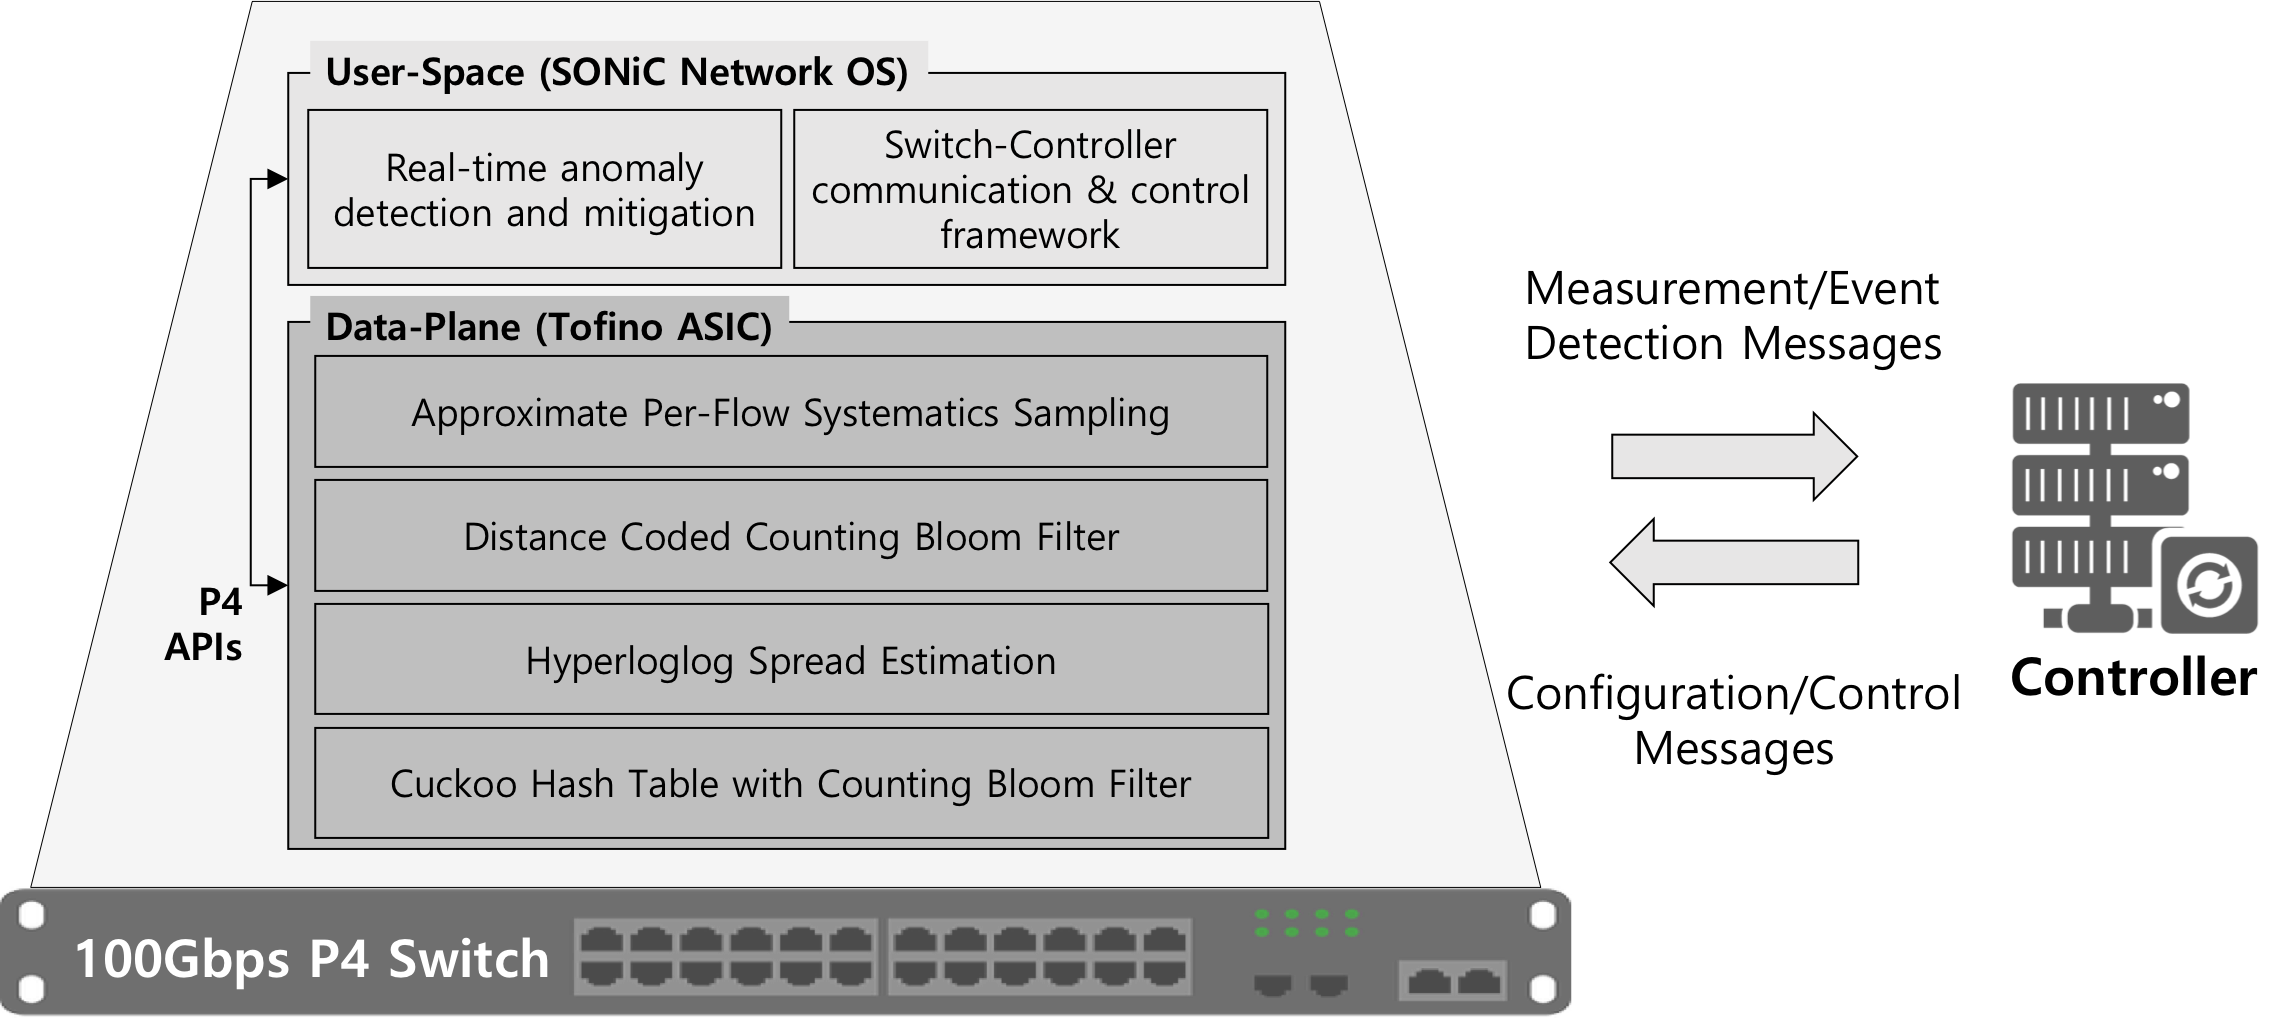
\includegraphics[width=0.8\textwidth]{fig/Vision.png} 
%   \caption{The high-level designs and goals of future research}
% \end{figure}

% The primary focus of my further research is to enable in-data-plane scalable traffic measurement and timely detection. Figure 1 shows the vision of my further research. The eventual goal of this research is not only proposing in-data-plane traffic measurement data structures and algorithms but also building a complete network device communication system that supports a network-wide measurement to deal with more comprehensive problems, such as network traffics engineering and anomaly detection. The algorithms are expected to be implemented in the commercial switch using data-plane programmable features of Intel's Barefoot Tofino ASIC. Moreover, the system-wise designs will strictly follow the state-of-the-art standards and contributed to the commercial/opensource switch system projects. 



% \BfPara{Thrust 1: Sketch-based Flow Sampling/Counting Technology}
% At the core of our system, we proposed a highly scalable and efficient in-data-plane per-flow sampling/counting algorithm to enable fine-grained (5-tuple) flow measurements under a high-speed and high-volume environment. Different from other sketches, our sketch is characterized as a low-cost data structure that can fit into a memory-constrained switch device and guarantees online performance. As known, sampling is a powerful tool to reduce the processing overhead in various systems. However, the wildly used Simple Random Sampling (SRS) approach samples packets over an aggregated data flow (defined by switch port or VLAN) and provides pool accuracy for different fine-grained flows (defined by the 5-tuple). 
%  %Figure 2 (right figure) shows the accuracy of our core algorithm, namely SketchFlow. For each flow, the fraction of the sampled packet number over the flow sizes almost equivalent to the sampling rate of 1/p. Moreover, the variance of SketchFlow is much smaller than the simple random sampling scheme (left figure).
% We stress that the scalable fine-grained per-flow measurement is a missing function in most of the commercial switches, because of the constrained resources. The SRS approach was an alternative but is barely used in practice due to poor accuracy. Our sampling approaches will ensure the accuracy of 2nd-Order-statistic; even when the collected subpopulation is dreamily smaller than the full population data. With our core algorithms, we opened new potentials to achieving fine-grained traffic engineering and anomaly detection using real-time provided fine-grained per-flow statistics. 

% % \begin{figure}
% %   \centering
% %   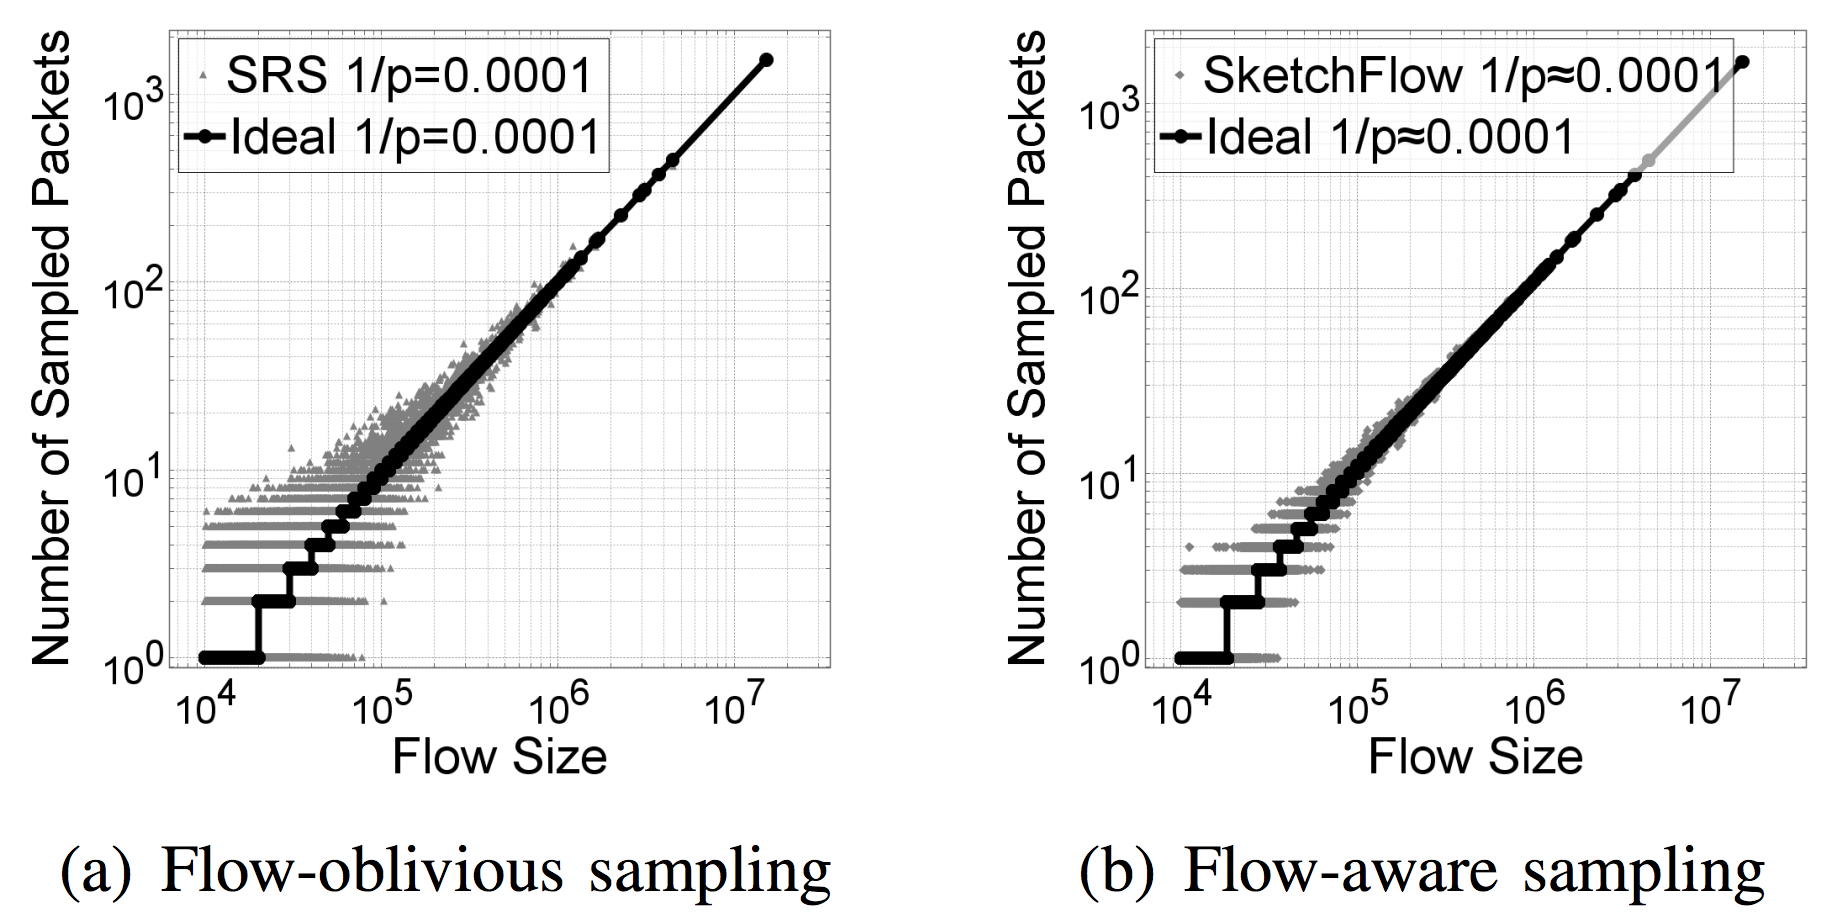
\includegraphics[width=0.8\textwidth]{fig/fig2.png} 
% %   \caption{Simple Random Sapling (SRS) vs. Approximated Per-flow Sampling (SketchFlow) vs. Exact Per-flow Sampling (Ideal).}
% % \end{figure}

% \BfPara{Thrust 2: Per-flow Spectral Density Distribution Measurement Technology} 
% In this thrust, we focus on the sketch saturation problem. As discussed above, sketches can maximize the efficiency of memory usage but eventually will be saturated by accumulated inflex information. One way to solve this problem is to recycle the memory space of inactive flows, which is very hard because the bit positions are not dedicated to individual flows. The other way is to mitigate the per-flow memory usage of the sketch. Instead of increasing bit position occupation to sketch the volume of flows, we use a computational distance to indicate the volume of flows, namely Distance-Coded Bloom Filter. In this way, we can minimize the memory space assigned for each flow to scale up the flow counting and retention capacities.

% \BfPara{Thrust 3: Per-flow Spread Distribution Measurement Technology}
% Spreader detection is essential in terms of anomaly detection, such as spammer detection, Distributed Denial-Of-Service (DDoS) attack. Although the estimation of spreader can be driven by spectral density distribution, however, it is impractical to be placed in data-plane because of the computational overhead of its operations (extensive memory read). Moreover, given that the most critical attacks (\eg DDoS attack) usually generate a high volume and high entropy traffic within a short time, the measurement and detection are highly required to be lightweight and can be performed in a timely manner. In this thrust, we mainly focus on designing an in-data-plane decodable spreader detector that can be deployed in commercial switches (data-plane programmable switch) to detect spreader-related anomalies in real-time. 

% \BfPara{Thrust 4: Scalable Flow Record Hash Table} 
% %Flow record table can be found in all commercial switches and routers, which are usually stored in TCAM  or SRAM for switching or routing purposes. 
% %NetFlow uses TCAM to parallel match flow IDs and lookup the corresponding actions or updates the flow counting volumes in the SRAM.
% %However, the number of entries in the table cannot be large because those types of memories are quite expensive. 
% Flow record table is stored in fast-but-small TCAM or SRAM for switching purposes. 
% For scalability, we can put the flow record table in DRAM instead of the expensive memory. 
% %(i.e., an incentive to cost-effectiveness). However, there is a speed issue for the In-DRAM flow record table: a packet arrival rate is too fast to handle in the DRAM, owing to the DRAM's slow access speed 
% Nevertheless, DRAM's slow access time
% (roughly ten times slower than TCAM and SRAM) and the hash collision is shortcomings. One way to compensate for the slow DRAM is to use sampling techniques to mitigate the influx rate of the hash table, which has been shown is efficient in our previous work (InstaMeasure; IEEE ICDCS 2019). However, a hash collision of the flow table is another problem. 
% To address this problem, we will design a sketch-guided cuckoo hash table that can drastically reduce the number of the access time of DRAM. The initial design of our new sketch is to use a counting bloom filter to indicate the horizontal location of the flow entry in the cuckoo hash table. Combining that with the vertical location information, we can access the flow record with minimum DRAM accesses. 
% %As shown in Figure 3, the DRAM access time of our initially designed flow record table is stably near one over time, which can minimize the computational overhead caused by the hash collision. 
% System-wise, we plan to fit the sketch into on-chip designed SRAM of data-plane (ASIC Switch) to reduce the flow entry locating the time and put the flow record table in the user-space DRAM. By doing so, we expect to achieve efficiency and scalability at the same time. 

% %  \begin{figure}
% %   \centering
% %   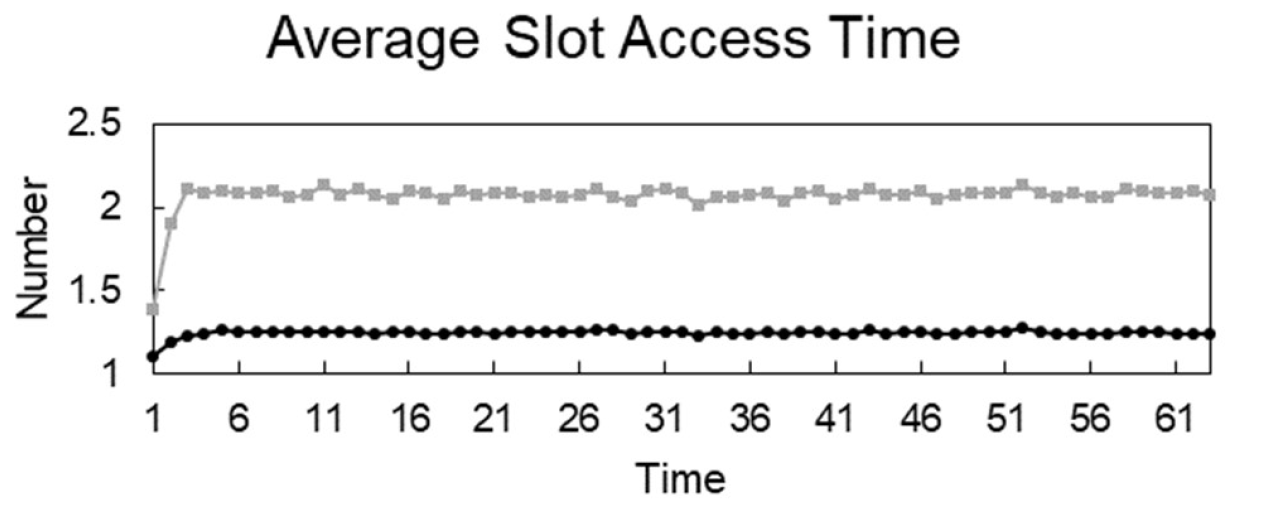
\includegraphics[width=0.8\textwidth]{fig/fig3.png} 
% %   \caption{The average DRAM access time of our hash table. Gray rectangles show the average DRAM access time of the original cuckoo hash table, and the Black circles stand average DRAM access time of our initially designed flow record table.}
   
% % \end{figure}
 

% \BfPara{Thrust 5: Onsite Anomaly Detection and Mitigation}
% Since the in-data-plane measurement is almost impossible using current technologies, traffic measurement is usually delegated by off-loading, sending sample packet headers, or accumulating temporally stored flow records to a remote server, leading to a Control Loop (delayed detection, mitigation, and control) between switches and controllers. In this thrust, we will focus on using a pre-defined rule sets to guide mitigation and control malicious flows in a local and timely manner (switch). By taking advantage of our proposed in-data-plane decodable data structures, the goal is to achieve an online detection of anomalies. For achieving more intelligent mitigation and control of networks, we expect to take advantage of machine learning techniques to dynamically predict and define the action sets.

% \BfPara{Thrust 6: Controller-and-Switch Communication Framework Integration}
% Our eventual goal is not only realizing the in-data-plane detection and mitigation but also achieving a network-wide defense and control. To do so, a centralized statistic collection server and control server are needed. The focus of this thrust is the use of fine-grained per-flow statistics from data-plane to achieve network-wide anomaly detection and information-driven precise traffic engineering. Previously proposed approaches are impractical to be integrated into an opensource switch system and software (\eg SONiC, Open Network Linux \etc). Instead of proposing a new framework from scratch, we will make efforts to embed our proposed data structures and algorithms into the opensource systems, and strictly following the state-of-the-art standards. For those designs that have not been standardized, we will actively make contributions to the future standard. 

\section{Potential of Attracting Funding}\vspace{-1mm}
The core of my research and associated thrusts are timely and useful to both academia and industry, with a high potential of attracting funding from industry, local state sponsors, and national funding agencies (\eg NSF, NRF). As mentioned earlier, top companies are actively working on blockchain systems and digital currencies. In 2020, I worked as a summer intern at Visa research. During my internship I was able to understand the ongoing trends in the industry and the future challenges that need to be addressed. My industrial collaborations will result in grants and gifts to extend the ongoing research on blockchain systems. Concurrently, I will be applying for grants and awards at Facebook with the objective to contribute the Calibra project. Similarly, I will propose the TEE-based {\em contactless} payment project to banks and financial sectors to seek sponsorship for the research. 

Blockchain systems and payment networks are highly researched areas in academia now days. In all major distributed systems and security conferences such as ICDCS and NDSS, there is a special track on the security of blockchains and payment networks. Considering the open challenges in the space there is a high potential of attracting funding from national funding agencies. In recent years, NSF and DARPA have funded several research projects on blockchain systems. My research opens new directions in security evaluation of blockchains and payments systems with a high likelihood of being sponsored by those agencies. 


% The core of my work and associated thrusts are quite timely, and will be of interest to both academia and the industry, and have the potential of attracting funding from the industry, local state sponsors, as well as national funding agencies (\eg NSF, NRF). In terms of academia, the recent network specialized major conference ACM CoNEXT (The 15th International Conference on emerging Networking EXperiments and Technologies, held between Dec 9 and Dec 12, 2019, and co-organized by my advisor) had a full session on the data-plane programmable networks. Moreover, top-tier conferences (ACM SIGCOMM and USENIX NSDI) intensively published programmable switch-related research work in recent five years. In terms of industry, recently, Intel acquired a major programmable switch company (Barefoot Networks), which sufficiently improved the penitential opportunities that programmable switches will become the new paradigms in the networking area. Potential sponsors of such work from industry will include the likes of Google, Cisco, Microsoft, Amazon \etc  


\section{Other research interests} \vspace{-1mm}
Besides my research in distributed systems security, I have actively worked in other research domains including \textbf{social media analysis} and \textbf{web security} (eCrime 2019). My future research will also extend in those domains 


\BfPara{Social Media Analysis} During my Masters, I worked on discovering the collusion networks and cyborgs on Twitter that were used to create a political divide among users. To detect those networks, I performed an extensive data collection of several notable Twitter accounts and (1) monitored their daily new followers and the {\em lock-step} retweeting activities of those followers. From the data and analysis, I uncovered various Twitter campaigns that were organized by collusion network to spread political narratives through trends and retweets. Through a deeper inspection, I discovered vulnerabilities in Twitter's account creating mechanism that allowed automated creation of fake accounts while bypassing the email authorization. I notified Twitter with my new findings and those vulnerabilities have been patched.  

More recently, I used Twitter data to determine public awareness regarding COVID-19 in the most affected countries. Using a large-scale data collection system, I crawled 46K trends and 622 Million tweets from the twenty most affected countries. Next, I performed a longitudnal study on the COVID-19 trends, the volume of tweets in those trends, and the user sentiment towards COVID-19 preventive measures. The results showed that in countries with a lower spread, Twitter users actively discussed the pandemic threat and the preventive measures. The study further showed that in countries with a higher spread, users exhibited a negative sentiment towards preventive measures. 

Based on my prior research experience, I will continue to use scientific tools to address social issues by using insights from social media platforms. In particular, using my training in security, I will try to detect hate campaigns and fake news that increase polarity in our social structure, making social media platforms unsafe for users. For this research, I will conduct a multi-disciplinary research in collaboration with the faculty of social science department to broaden the scope and impact our research.  

\BfPara{Web Security}


% \BfPara{Malware Analysis \& Detection (Work in progress)} Recent work has shown learning-based algorithms are vulnerable to adversarial examples, where a small perturbation in the input sample may result in misclassification. In this research, we systematically tackle the problem of adversarial examples detection in the control flow graph (CFG) based classifiers for malware detection. Unique to our approach, we use both density-based and level-based labels for CFG labeling to yield a consistent representation, a random walk-based traversal approach for feature extraction, and n-gram based module for feature representation. End-to-end, our approach representation ensures a simple yet powerful randomization property of the used classification features, making it difficult even for a powerful adversary to launch a successful attack. We also employ a deep learning approach, consisting of an auto-encoder for detecting adversarial examples, and a CNN architecture for detecting and classifying malware samples. To evaluate, we use a large dataset consisting of 16,814 IoT samples and demonstrate its superiority in comparison with state-of-the-art approaches. 

% \BfPara{IoT authentication protocol (Submitted to IEEE Transactions on Computers)} In this work, we introduce DigitalSeal, a hardware-based system with a protocol realization to authenticate Internet of Things (IoT) devices. DigitalSeal is a novel standalone hardware-based authentication tool that reads a barcode and displays a barcode data and its corresponding HMAC, which are used for authentication. DigitalSeal can manage cryptographic keys securely and provide data integrity in order to defend against Man-in-the-Middle (MitM) and Man-in-the-Browser (MitB) attacks. Moreover, DigitalSeal can be used in various applications, such as an authentication system or protocol, an online/offline transaction, a login session, and an IoT device authentication. Using DigitalSeal, we propose a new protocol for IoT device authentication, providing various security benefits, and reducing the burden of key maintenance for a large number of IoT devices. 
% %Our authentication protocol realization with DigitalSeal prevents unauthorized IoT devices from connecting to the user's gateway (an IoT home/enterprise network) and secures the communication between the IoT device and the gateway. 
% %Our system and associated protocol are both cost-effective and usable. According to our experiments, most users are able to obtain the authentication credential (the HMAC) within 3 seconds with more than 93\% accuracy using DigitalSeal. 

% \BfPara{Website Fingerprinting Defender (In INFOCOM 2020)} The onion routing (Tor) network is designed to provide privacy to users through end-to-end encryption. However, recent studies have shown adversaries are able to recognize the visited websites by analyzing network traffic patterns, known as Website Fingerprinting (WF) attacks. The success rate of WF attacks highly depends on the set of network traffic features used to build the fingerprint. Such features can be used to launch a machine/deep learning-based WF attack, which can break the existing state-of-the-art defense mechanisms. In this research, we used an adversarial learning technique to present a novel defense mechanism, Deep Fingerprinting Defender (DFD), against deep learning-based WF attacks. The DFD aims to break the inherent pattern of the Tor users' online activity through the careful injection of dummy patterns in specific locations in packet flow. We designed two configurations for dummy message injection, the one-way injection, and two-way injection. We conducted extensive experiments to evaluate the performance of DFD over both closed-world and open-world settings. %Our results demonstrate that these two configurations can successfully break the Tor network traffic pattern and achieve a high evasion rate of 86.02\% over a one-way client-side injection rate of 100\%,  a promising improvement in comparison with state-of-the-art adversarial trace's evasion rate of 60\%. Moreover, DFD outperforms its state-of-the-art alternatives by requiring lower bandwidth overhead; 14.26\% using client-side injection.


% %\BfPara{Keywords of Future Interests} Data-plane programmable switch, 6G, Satellite-based wireless communication, IoT protocol.




\end{document}
